\documentclass[letterpaper]{article}
\usepackage[submission]{aaai2027}
\usepackage{natbib}
\usepackage{graphicx}
\usepackage{booktabs}
\usepackage{amsmath}
\usepackage{amssymb}
\usepackage{url}

\urlstyle{rm}
\def\UrlFont{\rm}
\frenchspacing

\title{Audio-CVR: Automatic Curation and Reference-Aware Evaluation for Directional Audio Composed Video Retrieval}
\author{Anonymous Submission}
\affiliations{}

\begin{document}
\maketitle

\begin{abstract}
Composed video retrieval must first locate the intended context and then identify the candidate that satisfies the requested edit, yet aggregate recall conflates these abilities.
Audio-CVR is a non-speech, audio-primary diagnostic that intentionally retains the unchanged reference as a query-specific pre-edit negative within the same context.
Its automatic pipeline combines audio-grounded edit generation, directional verification, muted-video and ASR-shortcut screening, audiovisual consistency checking, sampled repeat auditing, and provenance control.
Exact own-reference masking changes only that candidate's score; target-over-reference accuracy, score margins, and error attribution then localize failures to the target--reference boundary.
On model-verified Full1000 (1,000 queries; 2,000 target/reference items), exact masking raises V+A+T R@1 by 84.5, 96.0, and 99.2 points for adapted E5-Omni, ImageBind, and retrieval-trained OmniEmbed. Temporal and spatial perturbations reduce exact identity but leave 27.0--84.0-point reference drops. Enabling audio for the E5 adapter raises mean R@1 across five seeds from 5.9\% to 12.8\% ($\Delta=6.8$ points; 95\% CI [5.2, 8.5]; Holm-adjusted $p=0.0018$), while audio reduces ImageBind and OmniEmbed R@1 by 9.2 and 1.0 points. OmniEmbed also shows a 14.0-point drop on OmniCVR. A partial blinded audit judged 34/50 queries valid; on those 34 cases, adapted V+A+T R@1 rises from 17.1\% to 93.5\% after exact masking.
Together, these diagnostics separate contextual retrieval from edit-direction satisfaction and show that audio availability does not imply audio utility.
\end{abstract}

\section{Introduction}

Composed video retrieval (CVR) asks a model to retrieve a target video from a gallery using a reference video and a textual modification.
Existing benchmarks establish the task, scalable data construction, and fine-grained evaluation \cite{ventura2024covr2,ventura2024covr,hummel2024egocvr}, with recent extensions to audio \cite{ji2026omnicvr,han2026cova}.
Yet an aggregate recall score alone cannot distinguish two qualitatively different failures: a model may fail to find the relevant context, or it may find that context but rank the unchanged reference above the target that actually satisfies the edit.

This distinction is particularly sharp for audio-primary edits under preserved visual context.
Consider a reference video showing a scene with piano music, paired with an instruction requesting guitar music.
The reference remains an excellent visual match, but it represents the pre-edit state; the target must preserve the scene while satisfying the directed sound change.
The unchanged reference is therefore not merely another distractor.
It is a query-specific negative control that is semantically close yet fails the modification condition.

Audio-CVR studies this failure mode directly.
We define the task around a directional audio edit, screen pairs for visual and transcript shortcuts, and retain the reference as a mandatory gallery item.
We then intervene on the same score matrix by masking only the current query's reference.
All other candidates and scores remain unchanged, making the difference a paired diagnostic of reference-target confusion rather than a comparison between two newly sampled galleries.

This construction intentionally creates a sharp boundary rather than an accidental two-choice task.
The other 1,999 gallery entries test whether a model retrieves the correct contextual neighborhood; the query's own reference tests whether it can select the post-edit state within that neighborhood.
Near-saturated R@1 after masking therefore localizes the dominant error to target--reference ordering.
It does not imply that the masked condition is a substitute benchmark or that retrieving context is itself difficult.

Our contributions are threefold.
First, we develop a multi-stage multimodal curation pipeline that isolates audio-primary directional changes through audio-only analysis, shortcut screening, audiovisual verification, provenance-aware deduplication, and source-disjoint splitting.
Second, we formalize the unchanged reference as a query-specific pre-edit negative and introduce exact paired masking, identity perturbations, and reference-specific attribution to expose directional failures hidden by aggregate recall.
Third, cross-model and cross-benchmark experiments reveal identity-sensitive pre-edit source anchoring and show that audio can either support the edit or reinforce the source, depending on representation and fusion.
The adapter is deliberately treated as a baseline rather than a model contribution.

\begin{figure*}[t]
  \centering
  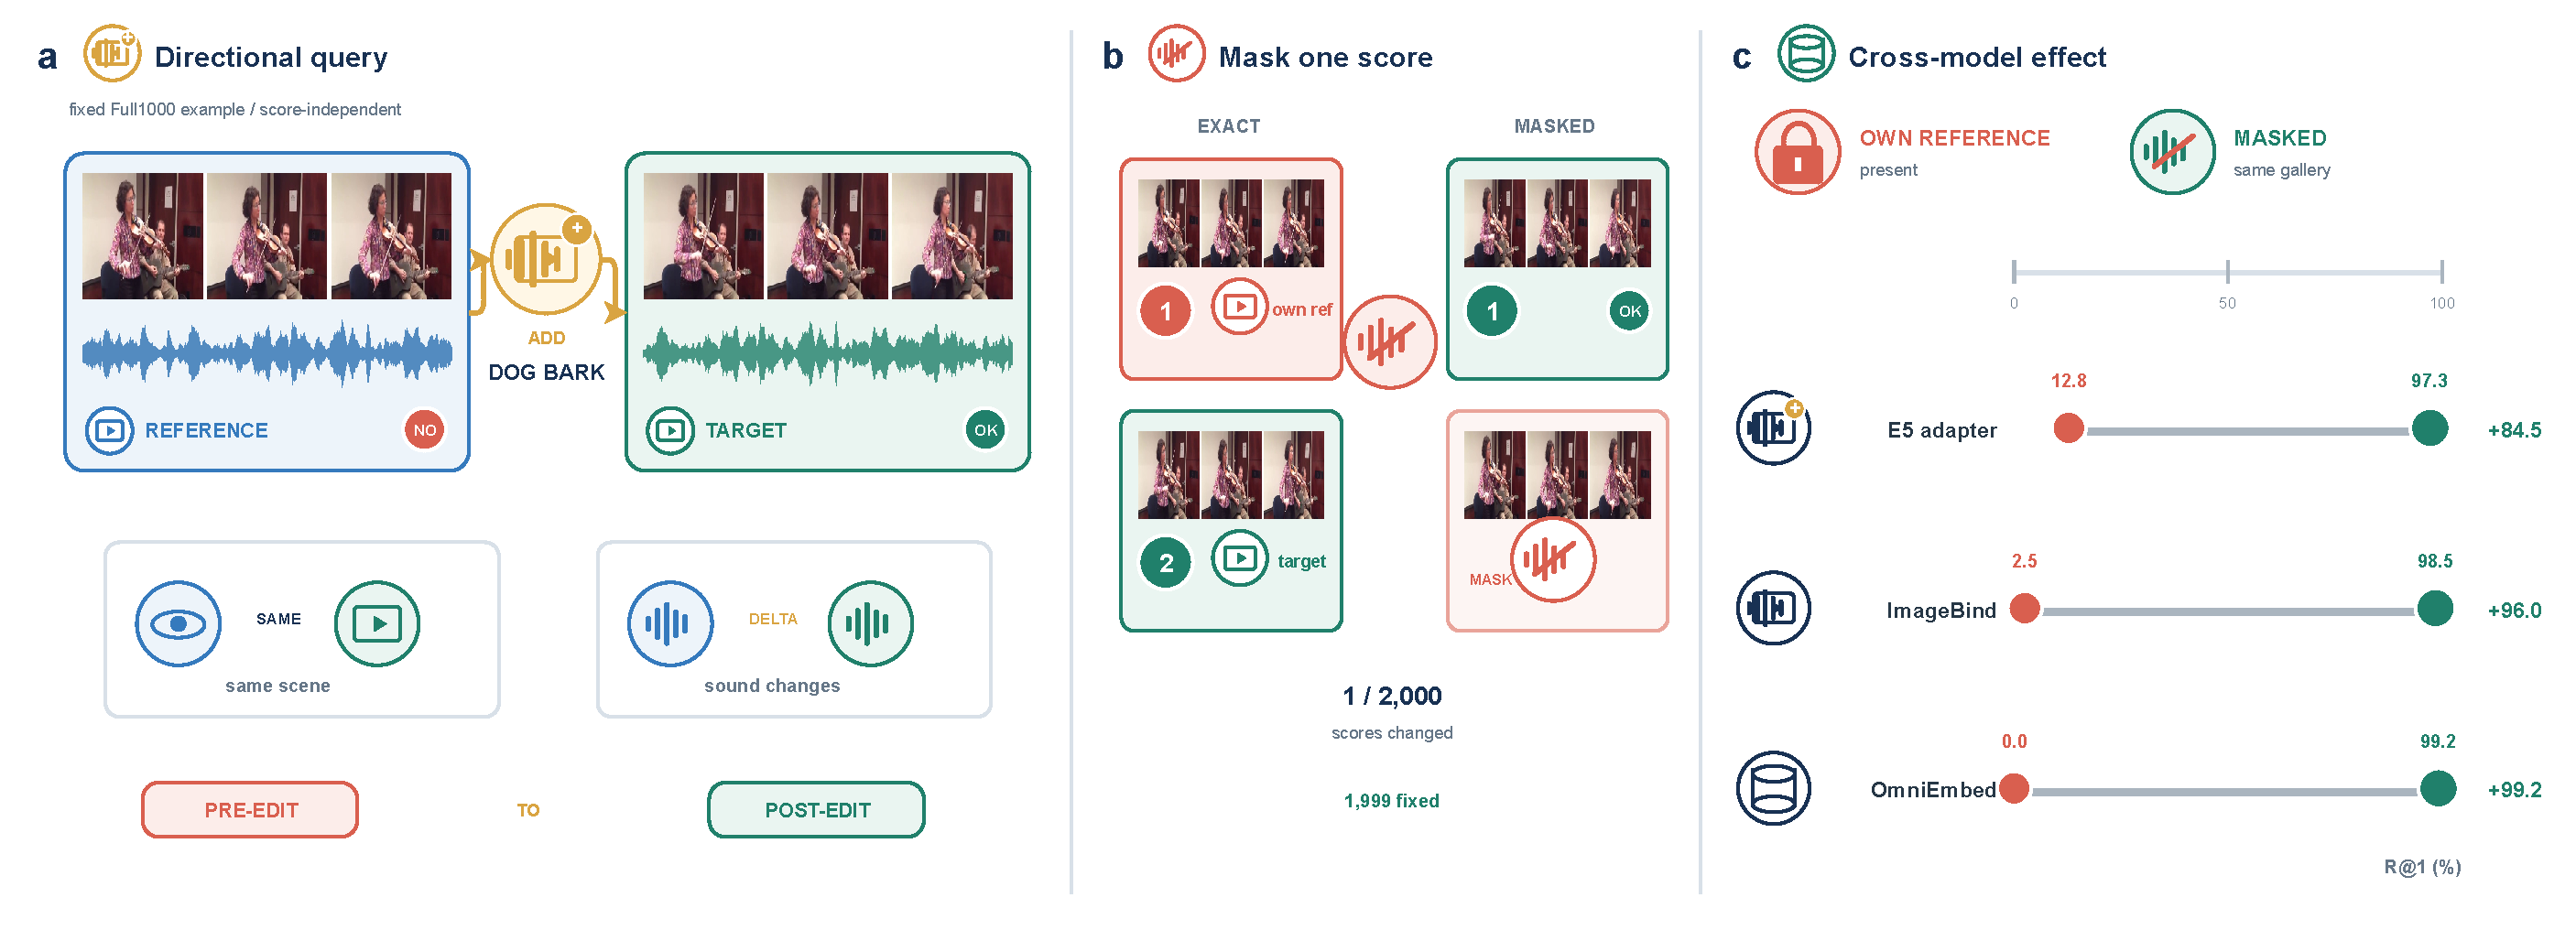
\includegraphics[width=\textwidth]{figures/generated/figure1_reference_confusion.pdf}
  \caption{\textbf{Audio-CVR isolates reference-target confusion.}
  (a) The reference preserves the desired visual context but does not satisfy the directed audio edit; the target does.
  (b) Exact masking changes only the score of the query's own reference, leaving the other 1,999 candidates and all other scores fixed.
  (c) The paired intervention exposes a cross-model preference for the pre-edit state without rebuilding the gallery.}
  \label{fig:reference-confusion}
\end{figure*}

\section{Related Work}

\paragraph{Composed retrieval.}
Composed image retrieval combines a reference image and modification text; CIRR broadened evaluation to real-life images and emphasized ambiguity in which content should be preserved \cite{liu2021cirr}.
CoVR transferred this formulation to video and introduced automatically mined web-video triplets together with an evaluation benchmark \cite{ventura2024covr2,ventura2024covr}.
EgoCVR subsequently focused on temporally fine-grained egocentric retrieval and demonstrated the value of diagnostic evaluation settings \cite{hummel2024egocvr}.
ReTrack identifies reference-oriented directional bias in composed features and mitigates it through directional anchor calibration \cite{li2026retrack}.
Audio-CVR addresses the complementary measurement problem: it makes the unchanged reference a controlled negative, intervenes on its score, and attributes errors specifically to that boundary.
These works motivate our use of paired source-target structure, but Audio-CVR isolates a different axis: a directional sound change under largely preserved visual context.

\paragraph{Audiovisual composed retrieval.}
OmniCVR establishes vision, audio, and text as first-class modalities and includes the source video and source-local distractors in its candidate gallery \cite{ji2026omnicvr}.
CoVA constructs audiovisual pairs and proposes modality-aware fusion for changes spanning visual and auditory content \cite{han2026cova}.
Audio availability does not imply audio utility.
CoVA reports R@1=25.9 for a direct trimodal fusion, below 28.8 for its V+T counterpart, whereas its learned selective fusion reaches 31.4.
AVIGATE similarly identifies blind audio incorporation as a source of suboptimal video representations and learns to suppress uninformative audio \cite{jeong2025avigate}.
We therefore do not claim to be the first audiovisual CVR benchmark or the first to place the source in the gallery.
Our contribution is a narrower diagnostic formulation: audio-primary directional isolation, exact source/reference masking, target-over-reference metrics, and reference-specific error attribution.
We treat audio benefit as an empirical question rather than a task assumption.

\paragraph{Omni-modal representations.}
E5-Omni targets cross-modal embedding alignment across text, image, audio, and video \cite{chen2026e5omni}.
ImageBind provides an independent shared embedding space for image, video, audio, text, and other modalities \cite{girdhar2023imagebind}.
OmniEmbed builds a multimodal retriever on Qwen2.5-Omni and is further trained for MultiVENT video retrieval \cite{xu2025qwen25omni,wu2025omniembed}.
OmniRet trains an omni-modal retriever on roughly six million query-target pairs spanning text, vision, and audio \cite{huynh2026omniret}.
VLM2Vec converts a vision-language model into an instruction-conditioned embedding model \cite{jiang2024vlm2vec}; our Audio-as-Text reproduction is retained only as a supplementary control.
We use these models as controlled evidence sources.
No ImageBind or OmniEmbed parameters are trained on Audio-CVR, and the E5 adapter is a lightweight task baseline; this coverage does not exhaust all recent specialized retrievers.

\section{Audio-CVR Task and Benchmark}

For a reference video $r$ with visual stream $v_r$ and audio stream $a_r$, and an edit instruction $t$, the goal is to retrieve target $y$ from gallery $\mathcal{G}$:
\begin{equation}
  y^* = \arg\max_{g \in \mathcal{G}} s\!\left(q(v_r,a_r,t), d(g)\right).
\end{equation}
We call the query input the \emph{reference}; OmniCVR calls the analogous pre-edit item the \emph{source}, whereas \emph{raw source} below refers only to the provenance video from which clips are cut.
The defining condition is a \emph{directional audio edit under preserved visual context}.
The reference should not satisfy the edit, the target should satisfy it, and pair curation screens out cases in which muted video alone identifies the target or the edit degenerates into transcript matching.

\paragraph{Operational validity.}
Let $m_t(x)$ denote whether video $x$ satisfies edit $t$ according to the staged reviewer.
An eligible triplet must satisfy $m_t(r)=0$ and $m_t(y)=1$, preserve the scene-level visual context, expose an audible difference, and pass a muted-video shortcut screen.
These are curation criteria rather than claims that every possible visual or linguistic cue has been eliminated.
The protocol does not assume that audio alone determines gallery identity: audio provides the primary changing evidence, while the visual stream specifies the preserved context.
The main benchmark excludes speech because transcript identity can otherwise dominate the intended audio-direction test.

\paragraph{Frozen evaluation sets.}
The Core150 subset contains 120 sound-event and 30 music queries.
The Full1000 benchmark contains 829 sound-event and 171 music queries.
It is automatically curated and model-verified, not a fully human-validated gold set.
The frozen Full1000 SHA256 begins with \texttt{70bd998c33bd}; the complete
digest and provenance are recorded in the release manifest.

\begin{table}[t]
\centering
\small
\setlength{\tabcolsep}{3.2pt}
\caption{Frozen Audio-CVR evaluation sets. Full1000 is automatically curated and model-verified; a partial blinded single-rater audit is reported separately. Neither split is presented as a multi-annotator gold set.}
\label{tab:benchmark}
\begin{tabular}{lrrrrr}
\toprule
Split & Queries & Sound & Music & Speech & Gallery \\
\midrule
Core150 & 150 & 120 & 30 & 0 & 1000 \\
Full1000 & 1000 & 829 & 171 & 0 & 2000 \\
\bottomrule
\end{tabular}
\end{table}

\paragraph{Composition and audit scope.}
Full1000 contains 510 Avatar, 275 VGGSound, 196 AVE, 10 WorldSense, and 9 VGG-MonoAudio queries. The final audit found no duplicate sample, source, or pair, no train/validation leakage, and no missing media. After freezing, all 78 requested repeat reviews were completed, with 79.5\% exact decision agreement and 85.6\% field-level agreement. This post-freeze audit remained observational: it neither changed benchmark membership nor informed selection. We therefore describe Full1000 as automatically curated and model-verified, not as a multi-annotator gold set. A blinded single-rater audit was stopped after 50 unique queries (51 displayed items), of which 34 were judged valid (68.0\%). Because only 23.2\% of the planned display sequence was completed, this is explicitly a partial quality audit rather than a prevalence estimate.

\paragraph{Staged freeze and provenance.}
Full1000 retains a fixed set of 516 previously constructed queries and adds 484 deterministically selected queries after either benchmark-level review or retained construction-stage Omni review, followed by a uniform deduplication and media audit.
The added data diversify the source pool with VGGSound \cite{chen2020vggsound} and AVE \cite{tian2018ave} event videos, while a small VGG-MonoAudio controlled supplement remains separately identified.
Selection uses review evidence, provenance, and stable hashes, never E5, ImageBind, or VLM2Vec retrieval scores.
The frozen manifest records every query's dataset, raw-source identity, media paths, review origin, and exclusion reason.

\paragraph{Gallery.}
Full1000 uses a shared gallery containing 1,000 targets and 1,000 unchanged references.
The with-reference condition therefore contains 2,000 entries; exact own-reference masking leaves 1,999 effective entries per query.
The final audit verifies target and own-reference indices and keeps every non-reference score fixed.
Typed hard negatives are reported as supplementary diagnostics and do not replace the mandatory reference comparison.

\section{Automatic Curation}

Figure~\ref{fig:curation} summarizes the construction procedure.

\paragraph{Clip and pair construction.}
Heterogeneous natural videos are normalized into 6--9 second clips, with 8 seconds as the default.
Each clip retains dataset, raw-source ID, source-group ID, temporal interval, and segment index.
Long videos yield sliding source windows; short videos reuse a valid full or tail interval.
Pair mining operates within these source groups and prioritizes clips whose visual context is similar but whose speech, music, or sound-event evidence differs.
This audio-first strategy avoids treating an arbitrary temporally adjacent pair as a valid edit.

\paragraph{Audio-grounded edit generation.}
The reviewer first receives only the reference and target audio.
It identifies a concrete audible delta and writes a directional edit from that evidence.
Keeping frames hidden at this stage reduces the chance that the instruction describes a visual change.
A second audio-only decision verifies the two logical sides of the edit: the reference must fail it and the target must satisfy it.
Ambiguous, generic, or contradictory edits are rejected rather than repaired using full-video context.

\paragraph{Shortcut and consistency gates.}
A muted-video reviewer tests whether the target can be selected from visual evidence alone; a full audiovisual reviewer then checks that the audio-grounded edit remains valid in context.
Speech-role and transcript-like checks screen ASR shortcuts, and speech is excluded from Full1000.
The stages intentionally answer different questions: audibility, direction, visual insufficiency, and contextual validity.
A pass at one stage cannot compensate for a failure at another.

\paragraph{Deduplication, review audit, and persistence.}
Canonical sample, unordered-pair, raw-source, and inverse-group identities are checked for duplicates before freezing and cross-checked against protected training and validation sources.
Review calls append atomic JSONL records containing the decision, confidence fields, reject reasons, reviewer profile, and media provenance.
Completed calls are therefore reused after interruption rather than regenerated.
The sampled repeat review measures stability but does not silently remove disagreements from the audit-only Full1000 selection.

\begin{figure*}[t]
  \centering
  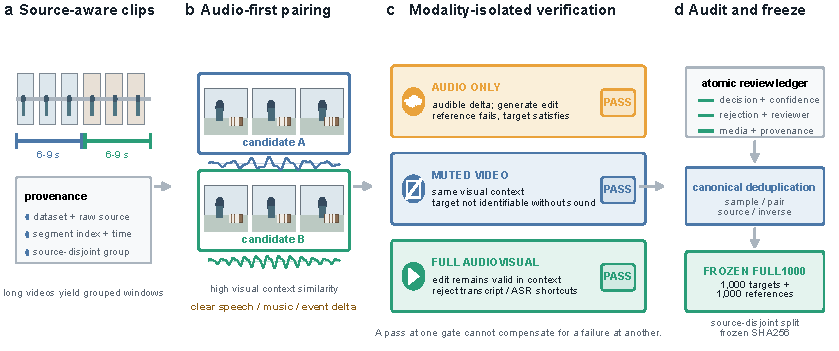
\includegraphics[width=\textwidth]{figures/generated/figure2_curation_pipeline.pdf}
  \caption{\textbf{Multi-stage multimodal automatic curation.}
  (a) Source-aware 6--9\,s clips retain stable provenance.
  (b) Pair mining favors preserved visual context and an explicit audible delta.
  (c) Audio-only, muted-video, and full-audiovisual reviewers test direction, visual shortcuts, contextual validity, and ASR shortcuts independently.
  (d) Atomic review records, canonical deduplication, and source-disjoint freezing produce the auditable Full1000 benchmark.}
  \label{fig:curation}
\end{figure*}

\section{Reference-Aware Evaluation}

\paragraph{Exact own-reference masking.}
Let $S_{ij}$ be the score of query $i$ against gallery entry $j$, and let $\rho(i)$ be the index of its own reference.
The masked condition is
\begin{equation}
  S'_{ij} =
  \begin{cases}
    -\infty, & j=\rho(i),\\
    S_{ij}, & \text{otherwise}.
  \end{cases}
\end{equation}
This intervention does not re-encode media, resample distractors, or remove other queries' references.
With-reference and masked-reference results therefore share the same score matrix.

\paragraph{Metrics.}
Alongside R@1, R@5, R@10, and reciprocal rank, we report target-over-reference accuracy
\begin{equation}
  \frac{1}{N}\sum_i \mathbb{1}[S_{i,\tau(i)} > S_{i,\rho(i)}],
\end{equation}
where $\tau(i)$ is the target index.
We also report the target-reference score margin, reference rank, reference-induced R@1 difference, and the fraction of top-1 errors in which the reference ranks first.
These metrics separate relevance from edit direction.

\paragraph{Interpretation of the intervention.}
The masked condition is not proposed as an easier replacement benchmark.
It asks a narrower counterfactual question: holding every other candidate and score fixed, would the target become top-ranked if the pre-edit state were unavailable?
A large increase therefore indicates that the errors are attributable to source-target ordering; it does not by itself establish open-world retrieval quality.
Conversely, a small increase would indicate that unrelated candidates, rather than the query's own reference, dominate the errors.

\paragraph{Reference-identity perturbations.}
Exact source inclusion can favor low-level self-matching.
We therefore replace only the query-specific gallery reference with one of three deterministic variants while leaving the query, target, other 1,998 candidates, and reference index unchanged: H.264/AAC transcoding; audiovisual trimming by 0.5\,s at each end; or a 90\% center crop resized to the original frame size while retaining the audio.
The ladder separates encoding identity, temporal/pixel identity, and residual pre-edit anchoring.

\section{Baselines and Experiments}

\paragraph{Models.}
We evaluate frozen E5-Omni, E5-Omni with a lightweight low-rank residual adapter, zero-shot ImageBind, and OmniEmbed-MultiVENT, a Qwen2.5-Omni checkpoint trained for multimodal video retrieval. The adapter has rank 32 and 688,131 trainable parameters over 3584-dimensional frozen embeddings. It is trained on 65 forward pairs plus 24 independently verified inverse pairs (89 directional instances), using 400 steps, a batch size of 8, and a learning rate of $10^{-3}$. Configuration selection uses only 28 validation queries under a one-standard-error rule. ImageBind uses fixed equal-weight arithmetic over normalized visual, audio, and text embeddings and receives no benchmark-specific training. OmniEmbed receives the same fixed retrieval instruction in every condition and is evaluated zero-shot, without Full1000 tuning. An Audio-as-Text VLM2Vec reproduction is retained as a supplementary control rather than treated as the official AudioVLM2Vec system.

\paragraph{Residual adaptation.}
For each query, document, and edit branch $b$, the adapter applies
\begin{equation}
  z_b(h)=\operatorname{norm}\!\left(h+B_b A_b h\right),
\end{equation}
where $A_b\!\in\!\mathbb{R}^{32\times3584}$ and
$B_b\!\in\!\mathbb{R}^{3584\times32}$.
Each $B_b$ is initialized to zero, so the initial representation exactly matches frozen E5-Omni.
Only these projections and three modality-temperature scalars are trained.

\paragraph{Zero-shot ImageBind.}
ImageBind independently embeds visual, audio, and text inputs in a 1,024-dimensional space.
We pre-register equal-weight normalized arithmetic: V+T uses
$\operatorname{norm}(V(r)+T(t))$ against $V(g)$, while V+A+T uses
$\operatorname{norm}(V(r)+A(r)+T(t))$ against
$\operatorname{norm}(V(g)+A(g))$.
No weight is selected on Full1000 and no ImageBind parameters are trained.

\paragraph{Retrieval-trained OmniEmbed.}
We use the public OmniEmbed-MultiVENT checkpoint, which adapts Qwen2.5-Omni for multimodal video retrieval \cite{xu2025qwen25omni,wu2025omniembed}.
V+T receives a silent reference video and a fixed retrieval instruction containing the edit; V+A+T receives the audiovisual reference with the same instruction.
Candidates are encoded with the matching silent or audiovisual mode.
The prompt is fixed before evaluation, and no Audio-CVR query is used for training or selection.

\paragraph{Research questions and controls.}
The experiments ask: (RQ1) how much top-rank failure is attributable to each query's own reference; (RQ2) how much survives identity-reducing perturbations; (RQ3) whether enabling audio improves directional ranking after task adaptation; and (RQ4) whether reference confusion transfers across model families and benchmarks.
All Full1000 modes share sample IDs, gallery indices, and validity masks.
The test set is accessed only after the E5 configuration has been selected using validation data, while ImageBind and OmniEmbed inputs are fixed before evaluation.

\paragraph{Modalities.}
Seven fixed modes isolate the available evidence: text-only against full audiovisual candidates, visual-only, audio-only, V+T, A+T, V+A, and V+A+T.
The primary audio comparison is V+A+T versus V+T.
The primary reference comparison is with-reference versus exact own-reference masking under the same modality and model.
No fusion weight or checkpoint is selected on Full1000.

\paragraph{Statistics.}
Adapter results use five fixed seeds.
Paired differences are assessed with 20,000 bootstrap samples and 20,000 paired randomization samples.
Queries are the independent units; for E5, each query's paired difference is averaged across seeds before query bootstrap and sign-flip randomization.
Per-seed top-1 changes use McNemar tests, and $p$-values for planned comparison families are corrected using the Holm procedure.
The query, gallery, and validity mask are held fixed within every paired comparison.

\begin{table*}[t]
\centering
\small
\setlength{\tabcolsep}{5.0pt}
\caption{Full1000 exact-reference results. R@1 and target-over-reference (T$>$R) are percentages; E5 adapter R@1 is mean $\pm$ std over five seeds. Masked R@1 changes only the current query's reference score.}
\label{tab:main-results}
\begin{tabular}{llrrrr}
\toprule
Model & Input & With-ref R@1 & Masked R@1 & T$>$R & Margin \\
\midrule
E5 base & V+T & 0.7 & 99.7 & 0.6 & -0.035 \\
E5 base & V+A+T & 0.3 & 99.7 & 0.3 & -0.031 \\
E5 adapter & V+T & 5.9 $\pm$ 1.0 & 98.3 $\pm$ 1.0 & 6.1 & -0.028 \\
E5 adapter & V+A+T & 12.8 $\pm$ 2.5 & 97.3 $\pm$ 1.9 & 13.2 & -0.021 \\
ImageBind & V+T & 11.7 & 99.3 & 10.8 & -0.008 \\
ImageBind & V+A+T & 2.5 & 98.5 & 2.5 & -0.023 \\
OmniEmbed & V+T & 1.0 & 99.2 & 0.1 & -0.057 \\
OmniEmbed & V+A+T & 0.0 & 99.2 & 0.0 & -0.055 \\
\bottomrule
\end{tabular}
\end{table*}

\paragraph{RQ1: Is top-rank failure concentrated on the own reference?}
Masking raises E5-adapter R@1 from 5.94\% to 98.28\% for V+T and from 12.78\% to 97.26\% for V+A+T. Across seeds, in 4,317 of 4,361 top-1 errors (98.99\%), the query's own reference ranks first. Frozen E5 exhibits the same pattern: its V+T and V+A+T R@1 values are 0.7\% and 0.3\% with the reference, but both reach 99.7\% after masking. ImageBind exhibits drops of 87.6 and 96.0 points; retrieval-trained OmniEmbed exhibits drops of 98.2 and 99.2 points. The adapted V+A+T target beats each designated visual, audio, and ASR hard negative in 100\% of comparisons, but beats its own reference in only 13.2\%. A historical mixed-gallery control places the reference above 83.3\% of same-source local candidates and 99.94\% of random candidates. \textit{Takeaway:} the models generally enter the correct contextual neighborhood but fail at the final target--reference direction boundary.

\paragraph{RQ2: Is the effect only exact self-matching?}
We replace only the own-reference item with a deterministic transcoded, temporally trimmed, or spatially cropped version. All 3,000 variants were generated without missing media, and all eight audited temporal/spatial variants preserved the pre-edit semantics. For adapted E5, the V+A+T reference-induced R@1 drop decreases from 84.5 points under exact inclusion to 42.9 after temporal trimming and 51.0 after spatial cropping. Residual drops remain 84.0/81.5 points for ImageBind and 60.0/45.8 for OmniEmbed. Exact identity is therefore a major component. \textit{Takeaway:} identity-reducing transformations leave substantial pre-edit anchoring, but this residual is not treated as standalone evidence of semantic edit reasoning.

\paragraph{RQ3: When does audio help?}
Under exact inclusion, V+A+T versus V+T raises adapted-E5 R@1 from 5.94 $\pm$ 0.99\% to 12.78 $\pm$ 2.55\% (+6.84 points; 95\% CI [5.16, 8.52]; Holm $p=0.0018$). R@5 and R@10 do not improve ($\Delta=-0.22$ and -0.06 points; Holm $p=0.640$ and $p=1.0$), localizing the gain to the top ordering boundary. The gain reverses after temporal and spatial perturbation ($-11.74$ and $-10.62$ points), where the reference audio remains highly source-identifying. Exact-condition audio also hurts ImageBind by 9.2 points and OmniEmbed by 1.0 point. Audio-only and A+T reach 12.88\% and 13.54\% R@1, neither below V+A+T at 12.78\%. \textit{Takeaway:} audio can reinforce either the requested edit or the pre-edit source; these results do not establish complete joint audiovisual semantic reasoning.

\paragraph{RQ4: Does the diagnostic transfer?}
Frozen and adapted E5, independently structured ImageBind, and retrieval-trained OmniEmbed all exhibit own-reference dominance on Full1000. On 1,000 OmniCVR audio-centered queries, OmniEmbed V+T rises from 0.1\% to 14.5\% after source masking; V+A+T rises from 0.0\% to 14.0\%. A partial blinded audit judged 34/50 completed unique queries valid (68.0\%); on those 34 human-valid cases, exact masking raises V+A+T adapter R@1 from 17.1\% to 93.5\%. The completed Core150 portion was 24/38 (63.2\%; Wilson 95\% CI [47.3, 76.6]); the audit is partial and does not estimate Full1000-wide validity. \textit{Takeaway:} source anchoring appears across retrievers, on an external benchmark, and on the audited human-valid subset.

\paragraph{Supplementary training control.}
Verified inverse augmentation is not a hidden source of the adapted-E5 gain: on Core150 it reduces R@1 from 22.9\% to 18.9\% ($\Delta=-4.0$ points, Holm $p=0.037$), despite improving the score margin. We retain this negative result and use the 89-instance model only as a fixed baseline.

\begin{table*}[t]
\centering
\small
\setlength{\tabcolsep}{6.0pt}
\caption{Reference-identity perturbation ladder on Full1000. Entries are reference-induced R@1 drops (masked minus with-reference, percentage points). Transcoding preserves content; temporal removes 0.5\,s from each end; spatial center-crops 90\% and resizes.}
\label{tab:reference-ladder}
\begin{tabular}{llrrrr}
\toprule
Model & Input & Exact & Transcoded & Temporal & Spatial \\
\midrule
E5 adapter & V+T & 92.3 & 84.1 & 32.6 & 41.5 \\
E5 adapter & V+A+T & 84.5 & 78.9 & 42.9 & 51.0 \\
ImageBind & V+T & 87.6 & 80.6 & 58.5 & 27.0 \\
ImageBind & V+A+T & 96.0 & 94.0 & 84.0 & 81.5 \\
OmniEmbed & V+T & 98.2 & 95.1 & 60.5 & 45.6 \\
OmniEmbed & V+A+T & 99.2 & 97.1 & 60.0 & 45.8 \\
\bottomrule
\end{tabular}
\end{table*}

\section{Discussion}

\paragraph{Why an intentionally sharp diagnostic is useful.}
Exact masking is not an alternative retrieval task: it is a paired intervention that separates contextual localization from edit-direction satisfaction.
High recall at larger $K$ and near-saturated masked R@1 indicate that the target often already lies in the retrieved neighborhood, while the unchanged reference controls the final ordering error.
This distinction is hidden when a benchmark reports only aggregate recall.

\paragraph{Identity and direction remain entangled.}
Transcoding leaves much of the effect intact, whereas temporal and spatial perturbations recover more target rankings.
The residual 27.0--84.0-point range is therefore evidence of identity-sensitive pre-edit source anchoring, not standalone evidence of semantic edit reasoning.
The perturbation ladder narrows the interpretation while preserving the central observation that the pre-edit candidate remains unusually competitive.

\paragraph{Audio availability and utility are different.}
The contrasting models reproduce the distinction drawn by CoVA and AVIGATE: unconditional audio fusion can preserve source-identifying evidence, whereas task-aware or selective composition may exploit edit-relevant evidence \cite{han2026cova,jeong2025avigate}.
Audio-CVR does not presume that sound must help.
It measures whether a composition mechanism can use sound to improve target--reference ordering without reinforcing the pre-edit source.

\section{Limitations and Conclusion}

Audio-CVR is intentionally narrower than general audiovisual composed retrieval.
\textit{Annotation scope.} Full1000 is automatically curated and model-verified rather than a multi-annotator gold set. The deterministic repeat review was completed after freezing (78/78; 79.5\% exact-decision and 85.6\% field-level agreement), but measures same-model stability rather than human consensus. The single-rater blinded audit is partial (50 unique queries; 68.0\% judged valid) and has no completed paired repeat for estimating intra-rater agreement. \textit{Benchmark scope.} The benchmark excludes speech and remains source-imbalanced, with 51\% of queries derived from Avatar; nine VGG-MonoAudio queries form a separately traceable controlled supplement. Review profiles are heterogeneous but recorded, strict same-source local negatives are unavailable at benchmark scale, and the task is a controlled diagnostic rather than a replacement for general AV-CVR. \textit{Interpretation scope.} The E5 adapter is a few-shot baseline trained on only 89 directional instances. ImageBind uses fixed equal-weight fusion, the Audio-as-Text VLM2Vec control is not the official AudioVLM2Vec system, and evaluation omits recent specialized retrievers such as OmniRet. One unrelated OmniCVR gallery video is excluded identically across OmniEmbed modes, without affecting a target or own reference. Identity perturbations do not fully separate identity from direction, so we claim identity-sensitive pre-edit source anchoring rather than a clean measure of semantic edit reasoning.
These limitations constrain benchmark scope, but do not alter the paired observation that removing one edit-inconsistent pre-edit candidate resolves most top-rank failures across multiple retrievers.
Within those boundaries, Audio-CVR makes measurable whether a retriever ranks the post-edit target above a context-matched pre-edit state.

\bibliography{references}

\end{document}
